\documentclass[12pt, a4paper]{scrartcl}

% CONFIG
\newcommand{\exptitle}{Pr:YLF Laser}  	    % long name of experiment
\newcommand{\exptitleshort}{Pr:YLF Laser}				 	% short name of experiment
\newcommand{\expdate}{22. und 23. Mai 2017} 				% date of experiment
\newcommand{\exptutor}{Dr. Katrin \textsc{Dulitz}}

% PACKAGES + MODIFICATIONS
\usepackage[german]{babel} %standard language stuff
\usepackage[T1]{fontenc}
\usepackage[utf8]{inputenc}
\usepackage{textgreek}

\usepackage[fleqn]{amsmath}  % math
\usepackage{amssymb}

\usepackage{graphicx} %graphics
\usepackage{float} 
\graphicspath{{img/}}
\usepackage{subfig}

\usepackage[section]{placeins}			% keep figures in section

\usepackage[automark,headsepline]{scrlayer-scrpage} %headings
\pagestyle{scrheadings}
\ihead{\exptitleshort}
\ohead{\pagemark}
\cfoot{}

\usepackage{hyperref}
\hypersetup{
    unicode=true,          % non-Latin characters in Acrobat’s bookmarks
    pdftoolbar=true,       % show Acrobat’s toolbar?
    pdfmenubar=true,       % show Acrobat’s menu?
    pdffitwindow=false,    % window fit to page when opened
    pdfstartview={FitH},   % fits the width of the page to the window
    pdfnewwindow=true,     % links in new window
    colorlinks=true,       % false: boxed links; true: colored links
    linkcolor=blue,        % color of internal links (change box color with linkbordercolor)
    citecolor=green,       % color of links to bibliography
    filecolor=magenta,     % color of file links
    urlcolor=blue          % color of external links
}

\usepackage[labelfont=bf,format=plain,singlelinecheck=false]{caption}
% bold captions
% to indent the caption use format=hang
% singlelinecheck=false avoids centering of single line captions

%\usepackage{chngcntr} % change behaviour of counters in different environments
%\counterwithin{figure}{section}  % number figures per section
%\numberwithin{equation}{section} % number equations per section
%\numberwithin{table}{section}    % number tables per section

\usepackage{enumerate} % better way to config enumerates

\setcounter{tocdepth}{2} % table of contents depth

\setlength{\parindent}{0pt} % no indent on new paragraph

\usepackage{pdfpages} % include pdf files

\usepackage{pdflscape} % landscape mode

% call Abschnitt and Unterabschnitt Kapitel with \autoref-command
%\addto\extrasngerman{
% \renewcommand{\sectionautorefname}{Kapitel}
% \renewcommand{\subsectionautorefname}{Kapitel}
% \renewcommand{\subsubsectionautorefname}{Kapitel}
%}


%%%%%
% Alter some LaTeX defaults for better treatment of figures:
    % See p.105 of "TeX Unbound" for suggested values.
    % See pp. 199-200 of Lamport's "LaTeX" book for details.
    %   General parameters, for ALL pages:
    \renewcommand{\topfraction}{0.9}	% max fraction of floats at top
    \renewcommand{\bottomfraction}{0.8}	% max fraction of floats at bottom
    %   Parameters for TEXT pages (not float pages):
    \setcounter{topnumber}{2}
    \setcounter{bottomnumber}{2}
    \setcounter{totalnumber}{4}     % 2 may work better
    \setcounter{dbltopnumber}{2}    % for 2-column pages
    \renewcommand{\dbltopfraction}{0.9}	% fit big float above 2-col. text
    \renewcommand{\textfraction}{0.07}	% allow minimal text w. figs
    %   Parameters for FLOAT pages (not text pages):
    \renewcommand{\floatpagefraction}{0.7}	% require fuller float pages
	% N.B.: floatpagefraction MUST be less than topfraction !!
    \renewcommand{\dblfloatpagefraction}{0.7}	% require fuller float pages
%%%%


% NEW COMMANDS
\newcommand{\grad}{\,$^\circ$C }
%\newcommand{\rb}[1]{$^{#1}$Rb}
%\newcommand{\difd}{\mathrm{d}}
%\DeclareMathOperator{\gaus}{gaus}
%\DeclareMathOperator{\cor}{cor}

% DOCUMENT SETTINGS

\title{\exptitle}
\subtitle{Master Laboratory Applied Physics}
%\author{Moritz Bitterling und Benjamin Rottler \\ Universität Freiburg}
\date{\expdate}

% DOCUMENT
\begin{document}

\hypersetup{pageanchor=false} %stop page numbering (hyperref) to prevent for double page numers
\newcommand{\HRule}{\rule{\linewidth}{0.5mm}}
\begin{titlepage}
\begin{center}
  \textsc{\Large Master Laboratory Applied Physics}\\[0.5cm]
  \HRule \\[0.5cm]
  { \huge \bfseries \exptitle}\\
  \HRule \\[0.5cm]
  \large \expdate\\[1cm]  
  \begin{minipage}{0.4\textwidth}
    \begin{flushleft} 
    \large
      Moritz \textsc{Bitterling}
    \end{flushleft}
  \end{minipage}
  \hfill
  \begin{minipage}{0.4\textwidth}
    \begin{flushright}
    \large
      Valentin \textsc{Vierhub-Lorenz}
    \end{flushright}
  \end{minipage}
  \\[1.5cm]
  \large 
  Betreuer: \exptutor \\[2cm]
  
\includegraphics[height=8cm]{img/logo_uni.pdf}
  \vfill
  \normalsize
  \textsc{Institut für Mathematik und Physik} \\
  \textsc{Albert-Ludwigs-Universität} \\
  \textsc{Freiburg im Breisgau}
\end{center}
\end{titlepage}
\thispagestyle{empty}


\newpage
\tableofcontents
\thispagestyle{empty}

\newpage
\hypersetup{pageanchor=true} %start page numbering again
\setcounter{page}{1} %set to page 1

\section{Versuchsziel}

lalala \cite{crc} 
\section{Physikalische Grundlagen}

\subsection{Funktionsweise eines Lasers}


Der Laser stellt eines der wichtigsten Werkzeuge der Experimentalphysik dar. Es gibt viele verschiedene Arten von Lasern, die grundsätzliche Funktionsweise ist jedoch immer ähnlich. Man benötigt zunächst ein aktives Medium in dem optische Übergänge stattfinden die zum emittieren von Photonen führen. Außerdem benötigt man eine optische Pumpe, die eine Besetzungsinversion im Medium erzeugt, wodurch sich mehr Atome im Zustand höherer Energie befinden. Dazu benötigt man mindestens drei Zustände, einen Grundzustand von dem aus die Elektronen in einen ersten angeregten Zustand gepumpt werden welcher mit möglichst kurzer Lebensdauer in einen weiteren angeregten Zustand etwas niedriger Energie fällt, der eine möglichst lange Lebensdauer besitzt. Dies verhindert, dass die Photonen des Laserlichts nicht direkt wieder absorbiert werden und Atome im niedrigen Zustand anheben. Zusätzlich benötigt man einen Resonator der Photonen mit einer bestimmten Energie und Impuls in den Laser zurückkoppelt. Diese Photonen regen dann Atome dazu an in den niedrigeren Zustand zu fallen und dabei ein Photon mit gleicher Energie und Impuls zu emittieren. Das führt zu dem gewollten monochromatischen und kohärenten Licht.
Wenn mehrere verschiedene Übergänge zur Verfügung stehen wird die Wellenlänge des Lasers durch die minimalsten Verluste, sowie die Wirkungsquerschnitte der Übergänge bestimmt. Die Verluste sind hierbei vor allem vom Resonator beeinflusst zum Beispiel über die Reflektivität der Spiegel.



\subsection{Stabilitätskriterium des Resonators}


Ein Resonator ist stabil, wenn ein Strahl auch nach beliebig vielen Reflexionen den Resonator nicht verlässt. 
Mit Hilfe von Matrizenoptik lässt sich dafür das Stabilitätskriterium eines Resonators
ableiten:

\begin{equation}
0\leq g_1 \cdot g_2 \leq 1
\end{equation}

wobei $g_1=(1-\frac{L}{R_1})$ und $g_2=(1-\frac{L}{R_2})$ mit den Krümmungsradien der Spiegel $R_{1/2}$ und dem Abstand der Spiegel L. In diesem Versuch verwenden wir hauptsächlich einen hemisphärischen Resonator mit einem Spiegel mit einem Krümmungsradius
von 100\,mm, für die Frequenzverdopplung wird jedoch ein sphärischer Resonator benötigt mit 
einem zweiten Spiegel mit einem Krümmungsradius von 150\,mm.
In Abb.~\ref{img:stabkrit} sind die Verläufe von $g_1 \cdot g_2$ als Funktion des Abstands der Spiegel dargestellt. Daraus ergibt sich für den hemisphärischen Resonator ein stabiler Zustand für einen Abstand bis 100\,mm und für den sphärischen Resonator zusätzlich von 150\,mm bis 250\,mm.

\begin{figure}[H]
\begin{center}
  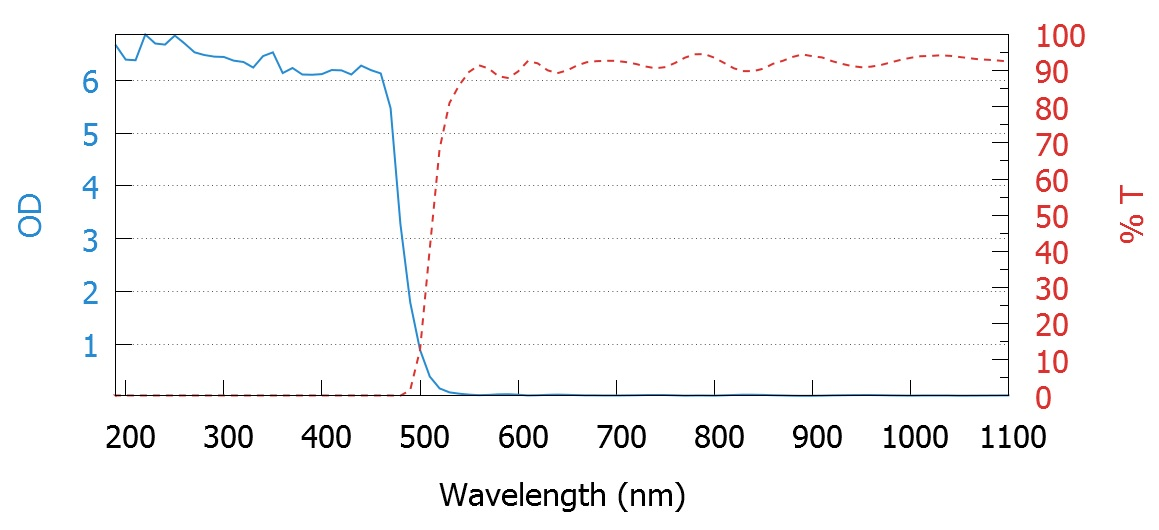
\includegraphics[width=.7\textwidth]{Schutzbrillen.png}
  \caption{Absorptions- (blau)  und Transmissionsspektrum (rot) der im Versuch
  verwendeten Laserschutzbrillen \cite{Versuchsanleitung}.}
  \label{img:stabkrit}
\end{center}
\end{figure}


\subsection{Eigenschaften des Pr:YLF-Lasers}

2. What are the specific characteristics of a Pr:YLF laser, i.e., why is it interesting to use a Pr:YLF
laser compared to other solid state lasers? In your answer, also make a comparison of the Pr:YLF
laser with the ruby laser and the Nd:YAG laser.

\begin{figure}[H]
\begin{center}
  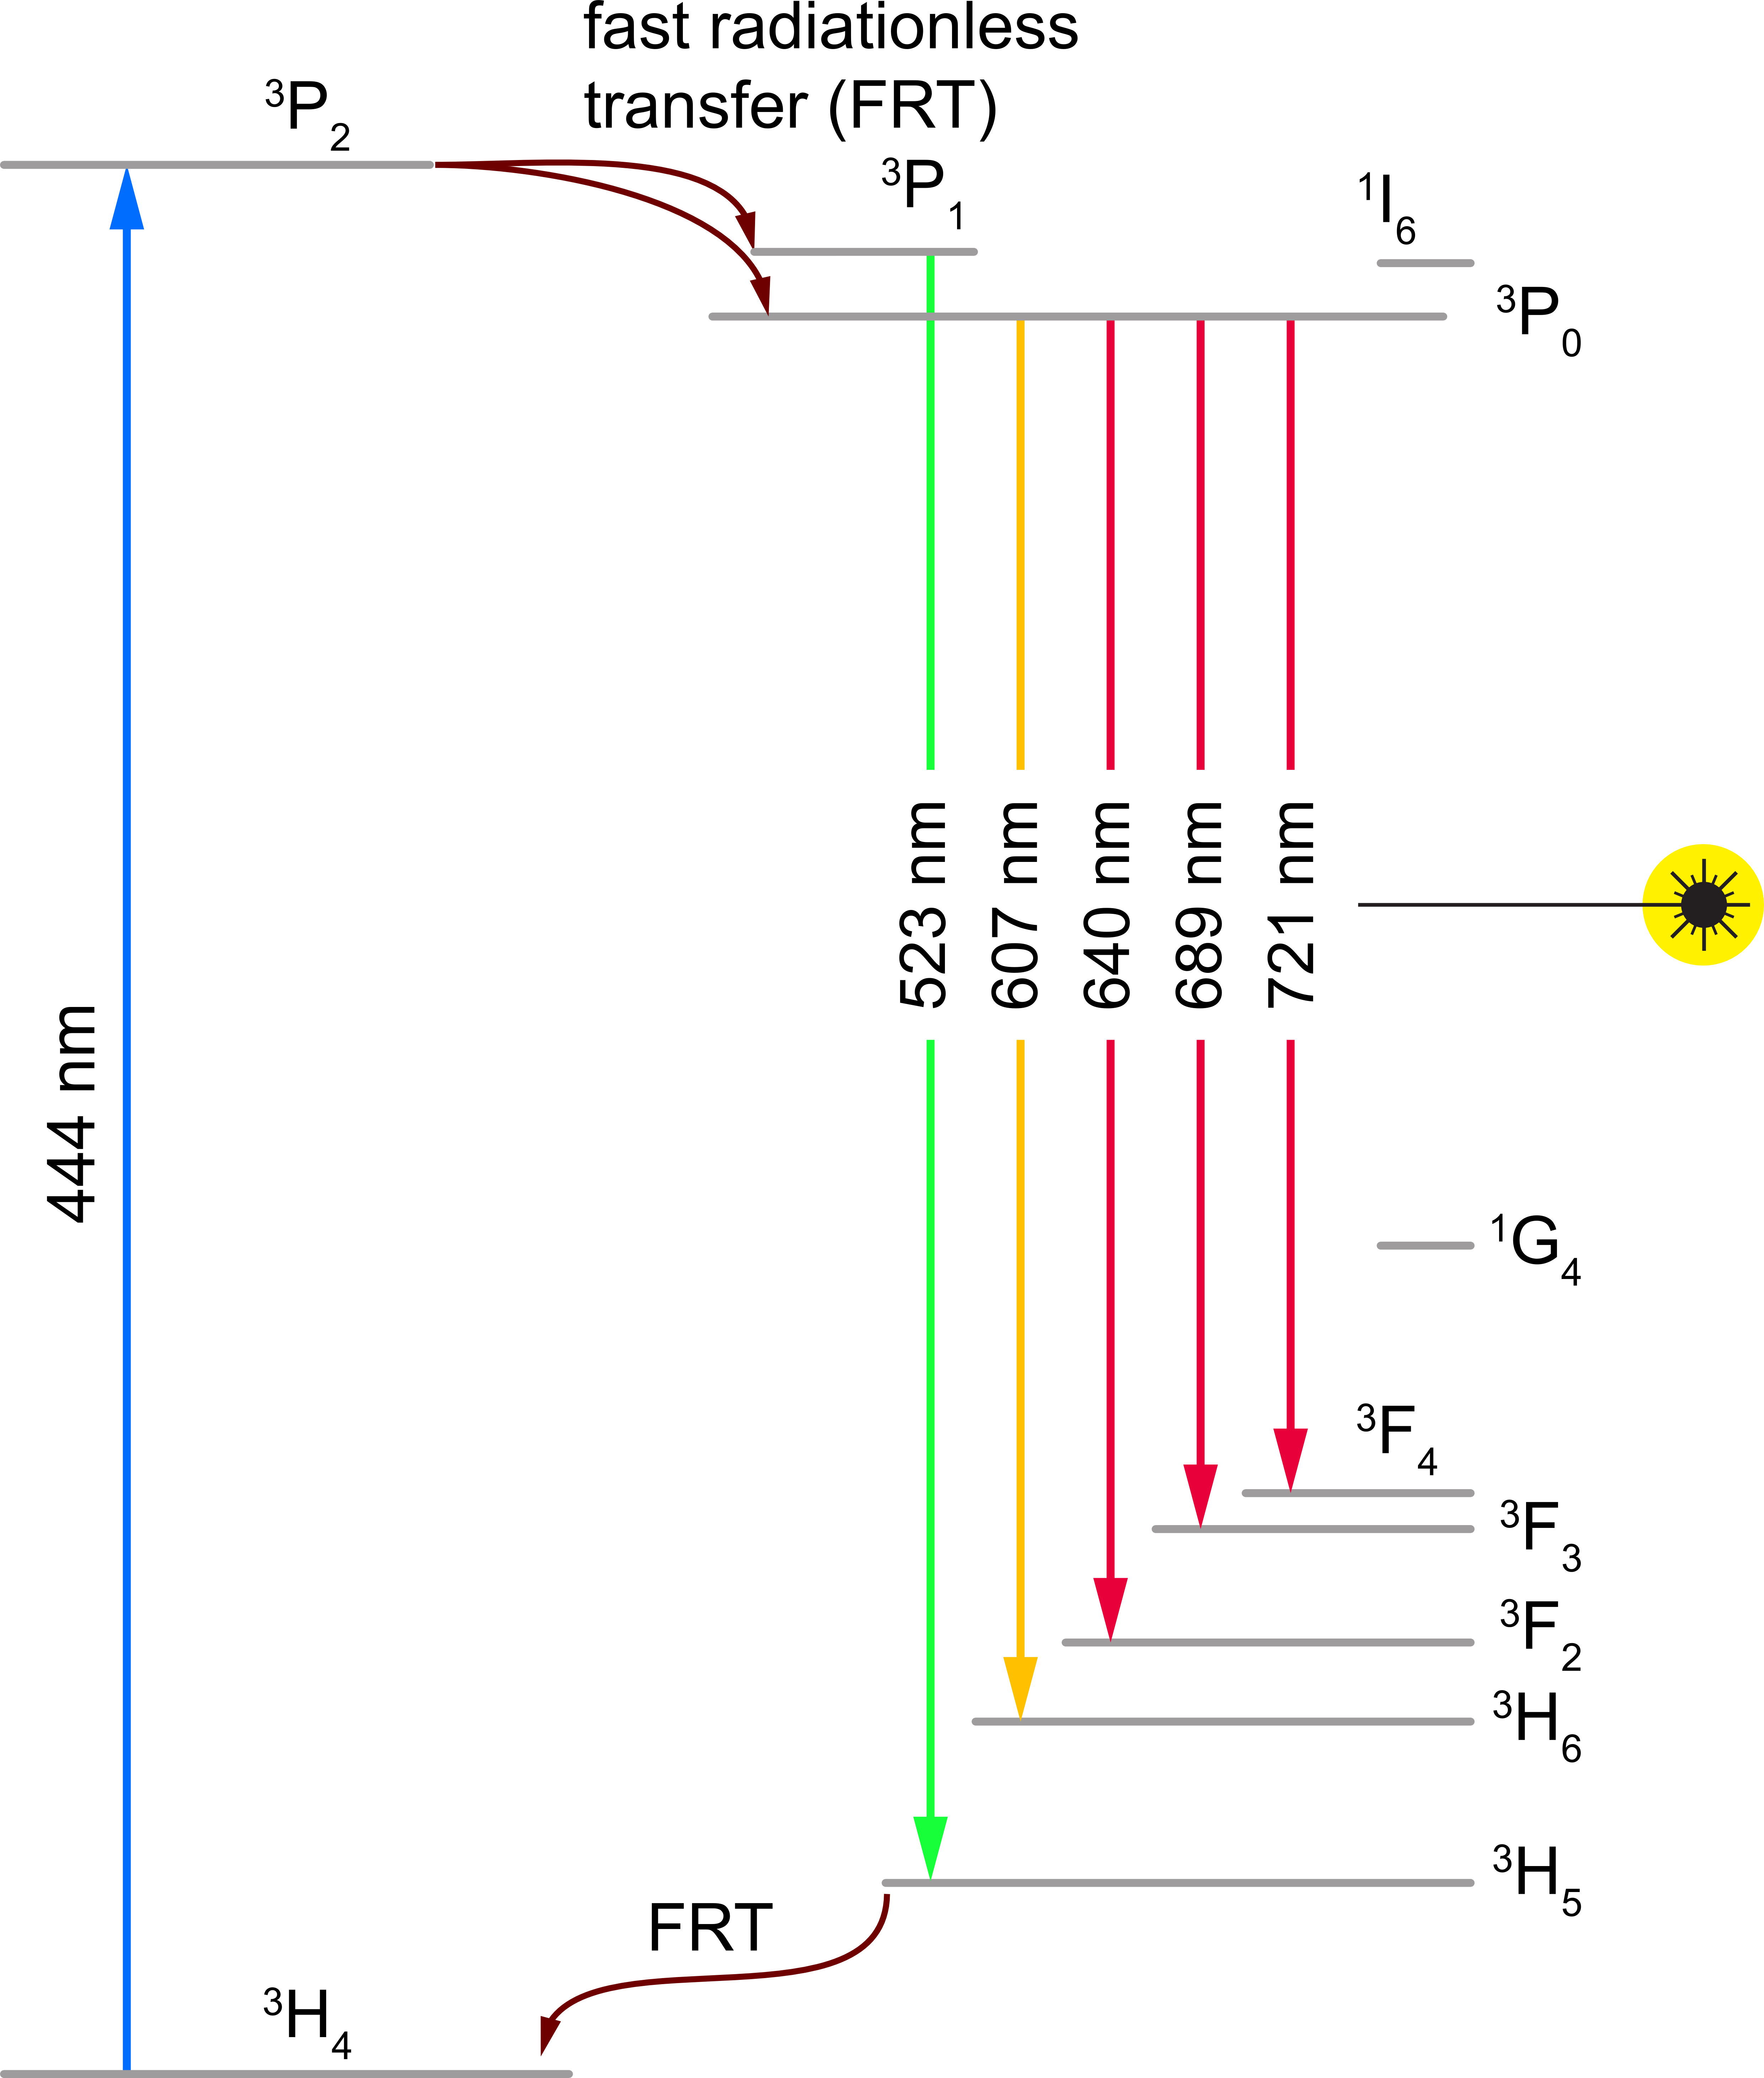
\includegraphics[width=.45\textwidth]{TermschemaPr3+.png}
  \caption{Termschema von Pr$^{3+}$ und relevante Übergänge für den Laserbetrieb
  \cite{Versuchsanleitung}.}
  \label{img:Termschema}
\end{center}
\end{figure}

\subsection{Wellenlängenselektion}


3. Compare the working principles of a birefringent tuner with those of a Littrow prism.


\subsection{Frequenzverdopplung}

4. How does second harmonic generation work and why does it have a low
efficiency?



\subsection{Laserschutzbrillen}

\begin{figure}[H]
\begin{center}
  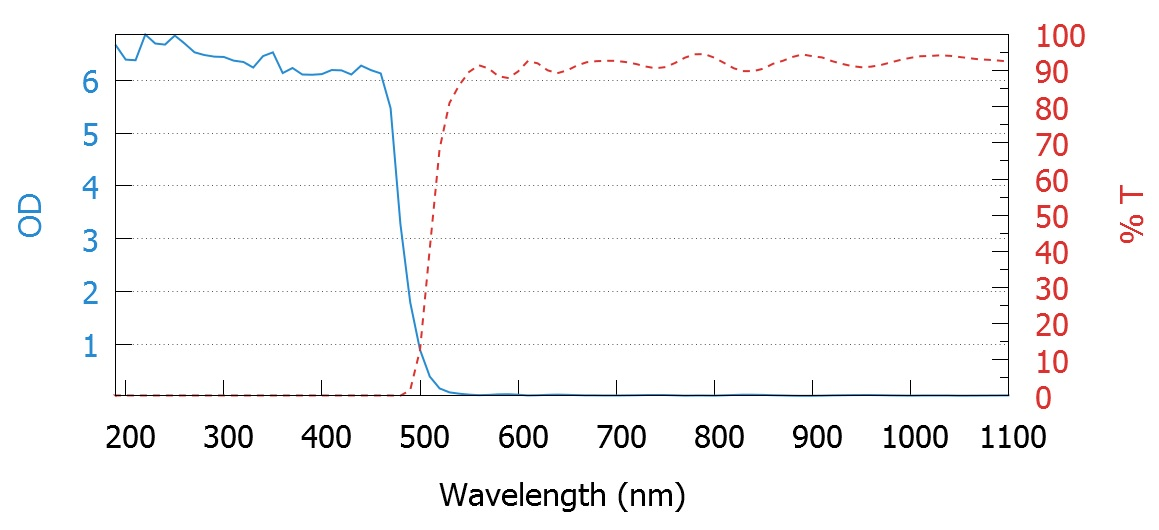
\includegraphics[width=.7\textwidth]{Schutzbrillen.png}
  \caption{Absorptions- (blau)  und Transmissionsspektrum (rot) der im Versuch
  verwendeten Laserschutzbrillen \cite{Versuchsanleitung}.}
  \label{img:Schutzbrillen}
\end{center}
\end{figure}

Abb.~\ref{img:Schutzbrillen} zeigt das Absorptions- und Transmissionsspektrum der
Laserschutzbrillen, die im Versuch verwendet werden.
Strahlung mit Wellenlängen unter 450\,nm wird um einem Faktor von mehr als $10^6$ abgeschwächt und
der starke blaue Pumplaser bei 444\,nm damit fast vollständig blockiert.
Bei Wellenlängen über 500\,nm beginnt eine signifikante Transparenz und über 550\,nm gelangt mehr
als 90\,\% des Lichts durch die Schutzbrillen,
so dass die Linien des Pr:YLF-Lasers beobachtet werden können.


\section{Aufbau, Durchführung und Auswertung}

\subsection{Charakterisierung des Pumplasers}


\subsubsection{Aufbau und Durchführung}

Pumplaser: Modulation mit 50\,\% über 700\,mA. Temperatur, Strom einstellbar

\subsubsection{Auswertung}

\begin{figure}[H]
\begin{center}
  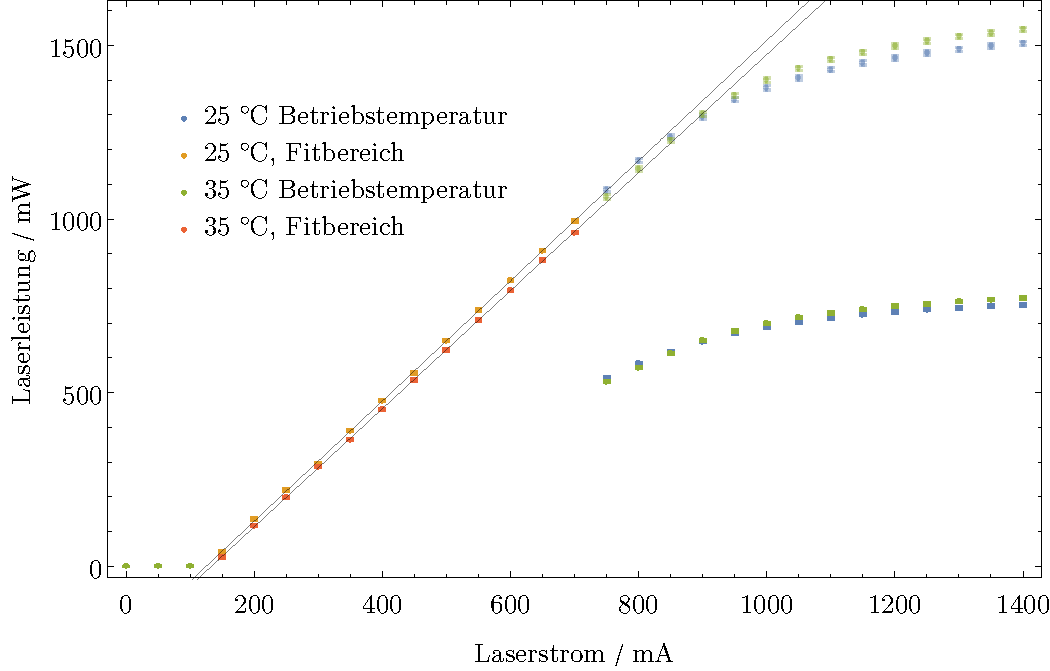
\includegraphics[width=\textwidth]{PI_blau.pdf}
  \caption{PI-Kennlinie des blauen Pumplasers bei 25\grad und 35\grad
  Betriebstemperatur. Der modulationsfreie Bereich wurde mit $y=a(x-b)$
  gefittet, um die Laserschwelle~$b$ und die Effizienz~$a$ zu bestimmen. Im
  Bereich der Modulation mit einer Pulsweite von 50\,\% über 700\,mA Laserstrom ist durch eine
  Multiplikation mit Faktor 2 angedeutet, bei welcher Leistung der Laser
  transient betrieben wird.}
  \label{img:PI_blau}
\end{center}
\end{figure}

Abbildung \ref{img:PI_blau} zeigt die beiden Kennlinien, die bei 25\grad und 35\grad Lasertemperatur
aufgenommen wurde.
Der Fehler der Laserleistung wurde aus der minimalen und maximalen Leistung abgeschätzt, die für die
einzelnen Messpunkte gemessen wurde.
Diese Schwankungen wurden mit höherem Betriebsstrom stärker.
Der Fehler auf den Laserstrom wird als vernachlässigbar klein angenommen.

 Nur der modulationsfreie Bereich von der Laserschwelle bis 700\,mA Laserstrom
zeigt einen linearen Verlauf.
Deshalb wurde der lineare Fit auf diesen Bereich beschränkt.
Da die Modulation des Lasers mit einer Pulsweite von 50\,\% stattfindet, hätte mit einer
Verdoppelung der Leistungen im Bereich über 700\,mA eine Erweiterung des Fitbereichs bis ca. 850\,mA
durchgeführt werden können. Erst bei Betriebsströmen über 850\,mA geht die Leistung deutlich in
Sättigung.
Tabelle \ref{tab:Fits_PI_blau} zeigt die Ergebnisse der beiden Fits.


\begin{table}[htb]
\caption{Ergebnisse der Fits der PI-Kennlinien des Pumplasers mit $y=a(x-b)$ von 150\,mA bis
700\,mA Laserstrom.}
\begin{center}
\begin{tabular}{|c|c|}
\hline
\textbf{25\grad} &  \\ \hline
$a$ & 1.730\,$\pm$\,0.005\,mW\,/\,mA \\ \hline
$b$ & 124.7\,$\pm$\,1.0\,mA \\ \hline
\textchi$^2$ & 16.0142 \\ \hline
\textchi$^2$/\,DoF & 1.60142 \\ \hline
 &  \\ \hline
\textbf{35\grad} &  \\ \hline
$a$ & 1.699\,$\pm$\,0.005\,mW\,/\,mA \\ \hline
$b$ & 133.0\,$\pm$\,1.0\,mA \\ \hline
\textchi$^2$ & 7.24023 \\ \hline
\textchi$^2$/\,DoF & 0.724023 \\ \hline
\end{tabular}
\end{center}
\label{tab:Fits_PI_blau}
\end{table}

\FloatBarrier
 
\subsection{Charakterisierung des Pr:YLF-Kristalls}

\subsubsection{Absorptionsspektrum}

Zur Bestimmung des Absorptionsspektrums des Pr:YLF-Kristalls wurde mit dem USB-Spektrometer ein
Referenzspektrum aufgezeichnet (Tageslicht vom Himmel), dann das Transmissionsspektrum des Kristalls
mit dem gleichen Licht aufgezeichnet und (vom Spektrometer) das Absorptionsspektrum als Differenz
berechnet.
Abb.~\ref{img:AbsSpec} zeigt das berechnete Spektrum.
Die Lage der Absorptionsmaxima ist eingezeichnet und in Tab.~ \ref{tab:AbsSpec} aufgeführt.

\begin{figure}[H]
\begin{center}
  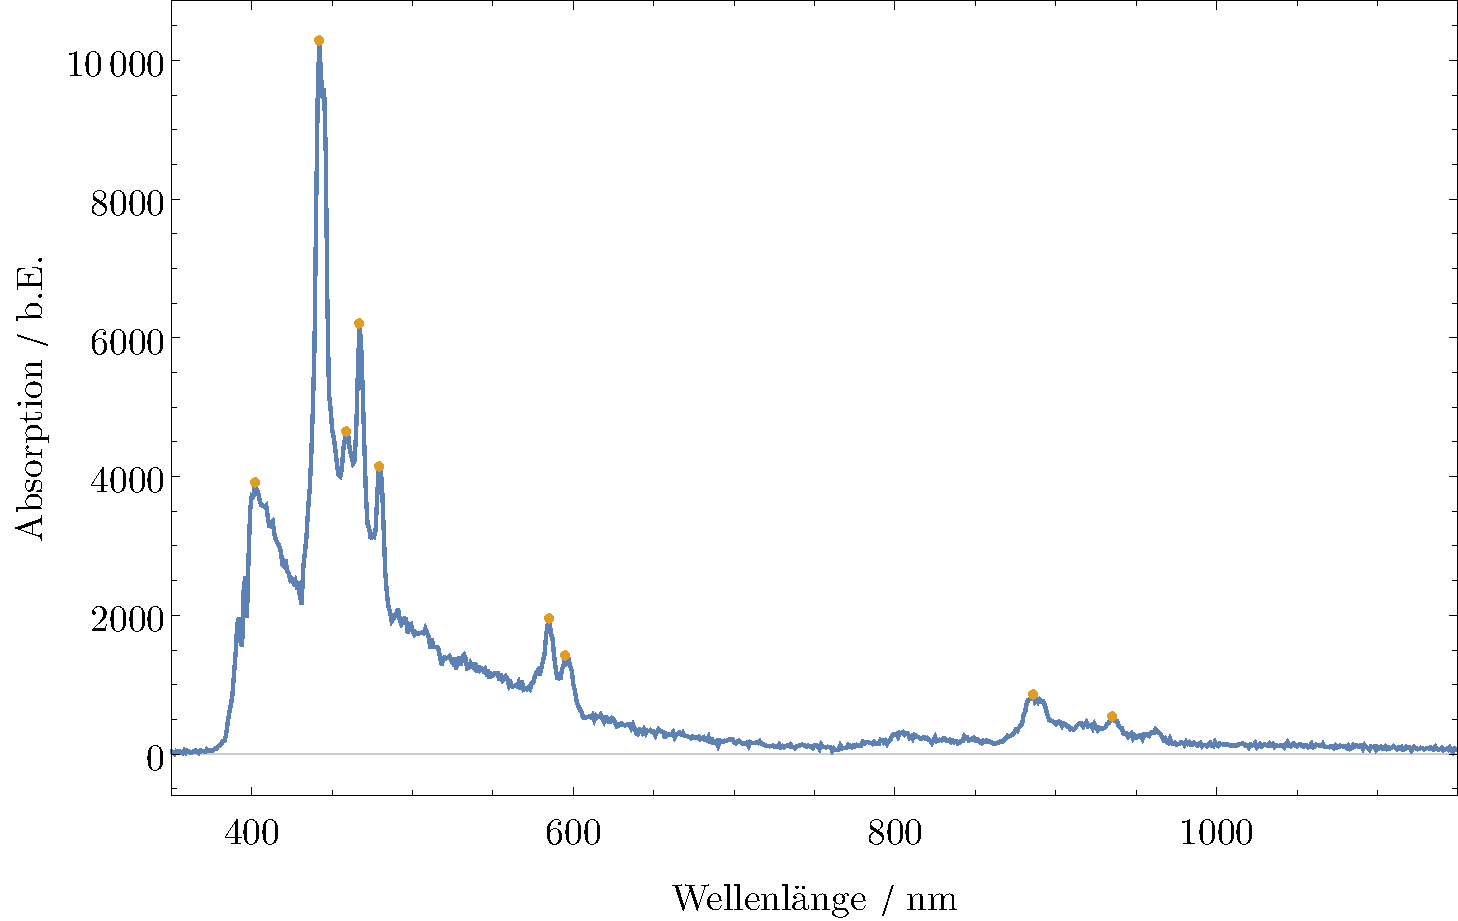
\includegraphics[width=\textwidth]{AbsSpec.pdf}
  \caption{Absorptionsspektrum des Pr:YLF-Kristalls und Position der deutlichen Maxima.}
  \label{img:AbsSpec}
\end{center}
\end{figure}

\begin{table}[htb]
\caption{Positionen und relative Intensitäten der Absorptionsmaxima im Spektrum des
Pr:YLF-Kristalls.}
\begin{center}
\begin{tabular}{|c|c|}
\hline
Wellenlänge / nm & Absorption / b.E. \\ \hline
402 & 3918.9 \\ \hline
442 & 10287.3 \\ \hline
459 & 4653.3 \\ \hline
467 & 6203.5 \\ \hline
479 & 4147.4 \\ \hline
585 & 1947.5 \\ \hline
595 & 1420.8 \\ \hline
886 & 850.9 \\ \hline
935 & 535.6 \\ \hline
\end{tabular}
\end{center}
\label{tab:AbsSpec}
\end{table}


\subsubsection{Emissionsspektrum}

\paragraph{Aufbau und Durchführung}
blablabla

\paragraph{Auswertung}

blablabla

\begin{figure}[H]
\begin{center}
  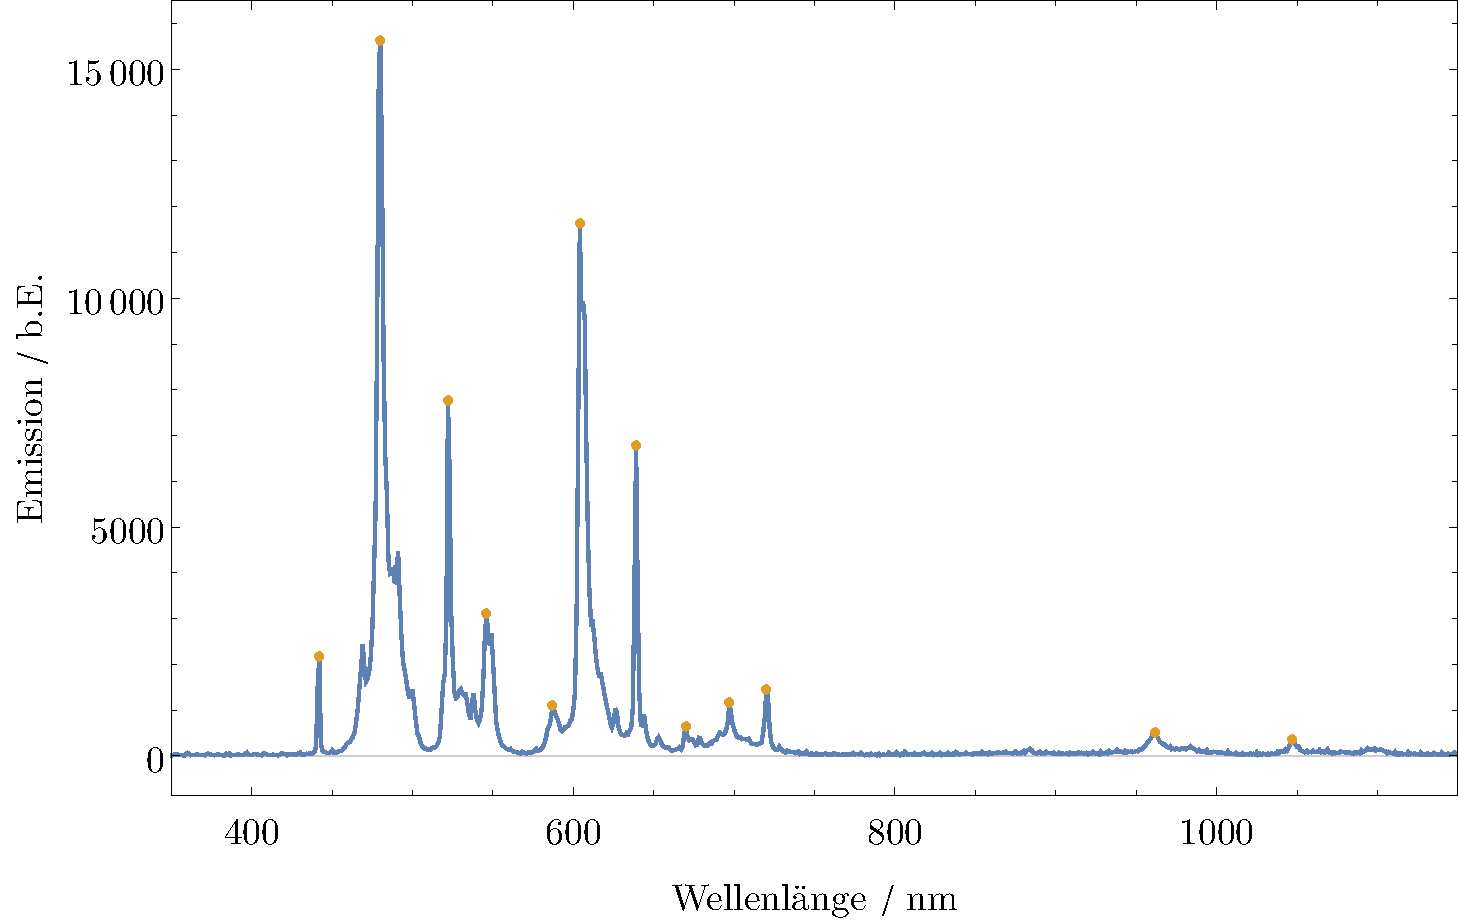
\includegraphics[width=\textwidth]{EmSpec.pdf}
  \caption{Emissionsspektrum des Pr:YLF-Kristalls und Position der deutlichen Maxima.}
  \label{img:EmSpec}
\end{center}
\end{figure}

\begin{table}[htb]
\caption{Positionen und relative Intensitäten der Emissionsmaxima im Spektrum des
Pr:YLF-Kristalls.}
\begin{center}
\begin{tabular}{|c|c|}
\hline
Wellenlänge / nm & Emission / b.E. \\ \hline
442 & 2168.6 \\ \hline
480 & 15633.9 \\ \hline
522 & 7761.3 \\ \hline
546 & 3115.6 \\ \hline
587 & 1099.0 \\ \hline
604 & 11627.5 \\ \hline
639 & 6787.0 \\ \hline
670 & 635.9 \\ \hline
697 & 1162.8 \\ \hline
720 & 1457.7 \\ \hline
962 & 508.6 \\ \hline
1047 & 366.7 \\ \hline
\end{tabular}
\end{center}
\label{tab:EmSpec}
\end{table}


\FloatBarrier


\subsubsection{Messung der Lebensdauer des angeregten Zustands}

\paragraph{Aufbau und Durchführung}

blabla

\paragraph{Auswertung}
Abb.~\ref{img:Lifetime} zeigt die Modulation der Laserspannung während der Messung und das
dazugehörige Fluoreszenzsignal, das von der Photodiode geliefert wird.
Das Photodiodensignal eines einzelnen Abschaltvorgangs ist auf Abb.~\ref{img:LifetimeFit} zu sehen. 
Als Fehler auf die Diodenspannung wird von der Spannungsauflösung des Oszilloskops
(0,2\,mV) ausgegangen und diese - unter Annahme einer Gleichverteilung der Fehler - durch
$2\sqrt{3}$ geteilt.
Der Fit des Signals erfolgt mit einer exponentiellen Abnahme mit Zeitkonstante~$\tau$ und
Untergrund~$U$. Das Fitergebnis ist auf Tab.~\ref{tab:Fit_lifetime} zu sehen.


\begin{figure}[H]
\begin{center}
  \includegraphics[width=.7\textwidth]{lifetime.png}
  \caption{Modulation des Lasers mit einem Rechtecksignal (gelb) zur Bestimmung der Lebensdauer der
  Fluoreszenz (blau, Messung als Spannungssignal der Photodiode).}
  \label{img:Lifetime}
\end{center}
\end{figure}


\begin{figure}[H]
\begin{center}
  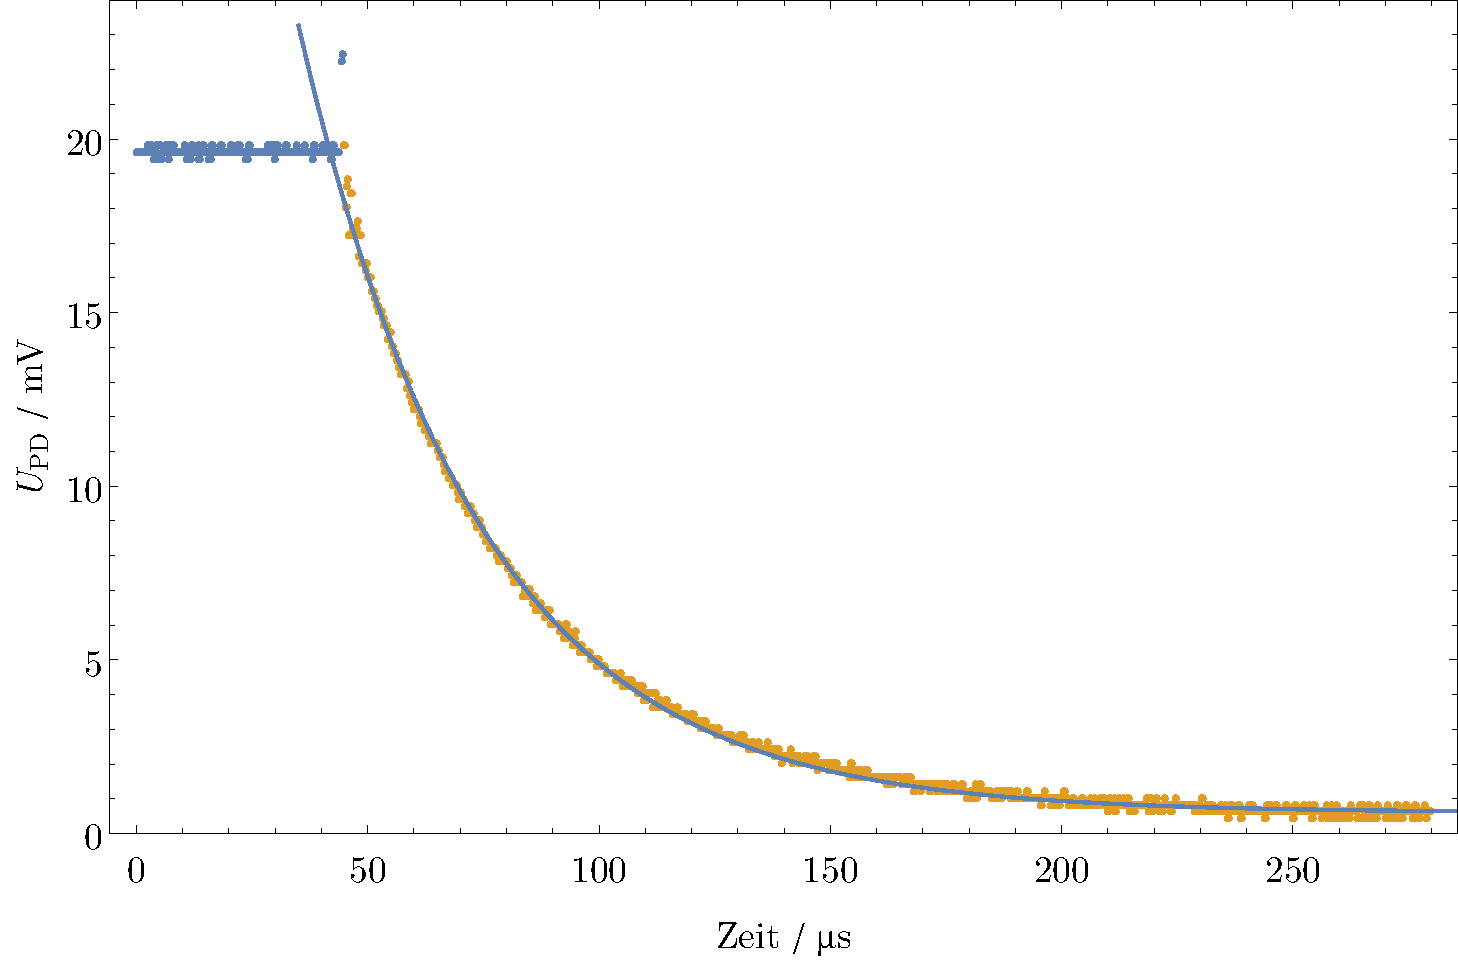
\includegraphics[width=.9\textwidth]{lifetime.pdf}
  \caption{Exponentieller Fit des Spannungssignals der Photodiode $U_{\text{PD}}$ zur Bestimmung der
  Lebenszeit des angeregten Zustands. Der Fitbereich ist gelb markiert, auf die Darstellung der geringen Fehler
  wurde verzichtet.}
  \label{img:LifetimeFit}
\end{center}
\end{figure}

\begin{table}[htb]
\caption{Ergebnisse des Fits der Fluoreszenzlebensdauer mit
$y=A\,\exp(-x/\tau)\,+\,U$.}
\begin{center}
\begin{tabular}{|c|c|}
\hline
$A$ & 55.65\,$\pm$\,0.21\,mV \\ \hline
$\tau$ & 39.01\,$\pm$\,0.10\,\textmu s \\ \hline
$U$ & 0.605\,$\pm$\,0.008\,mV \\ \hline
\textchi$^2$ & 527.875 \\ \hline
\textchi$^2$/\,DoF & 0.450021 \\ \hline
\end{tabular}
\end{center}
\label{tab:Fit_lifetime}
\end{table}


\subsubsection{Messung der absorbierten Leistung}

\paragraph{Aufbau und Durchführung}
blabla

\paragraph{Auswertung}
blabla
 
\begin{table}[htb]
\caption{Leistung am Leistungsmesskopf ohne Kristall im Strahlengang ($P_\text{ohne}$),
mit Kristall ($P_\text{mit}$), absorbierte Leistung ($P_\text{abs}$) und relative Absorption
$P_\text{abs}/P_\text{ohne}$ in Abhängigkeit von Lasertemperatur $T$ und Laserstrom $I$.}
\begin{center}
\begin{tabular}{|c|c|c|c|c|c|}
\hline
T / \grad & I / mA & $P_\text{mit}$ / mW & $P_\text{ohne}$ / mW & $P_\text{abs}$ / mW & Absorption / \% \\ \hline
25 & 400 & 114 & 427 & 313 & 73.3 \\ \hline
25 & 600 & 149 & 737 & 588 & 79.8 \\ \hline
25 & 800 & 87.4 & 532 & 444.6 & 83.6 \\ \hline
35 & 400 & 77.1 & 408 & 330.9 & 81.1 \\ \hline
35 & 600 & 105 & 718 & 613 & 85.4 \\ \hline
35 & 800 & 30.6 & 522 & 491.4 & 94.1 \\ \hline
\end{tabular}
\end{center}
\label{tab:Absorption}
\end{table}

\subsection{Charakterisierung des Lasers auf der roten Linie}

\subsubsection{Aufbau}



\subsubsection{Aufnahme der Kennlinien}



\subsubsection{Messung der Laserleistung mit Photodiode}



\subsubsection{Erzeugung verschiedener Moden}


\subsubsection{Messung des dynamischen Verhaltens}
\subsection{Wellenlängenselektion}

\subsubsection{Selektion über Reflektivität der Spiegel}

\paragraph{Aufbau und Durchführung}

bei gelber PI:
Messung mit kleinem power head
grün dabei bei kleinen Strömen


\paragraph{Auswertung}
blabla

\begin{figure}[H]
\begin{center}
  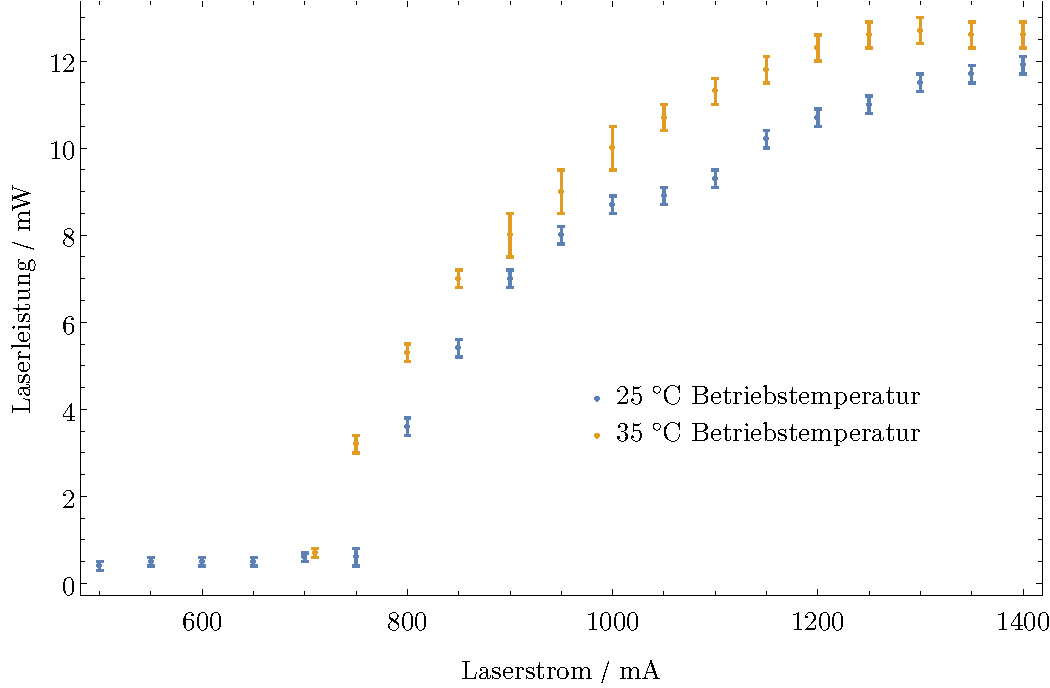
\includegraphics[width=\textwidth]{PI_gruen.pdf}
  \caption{PI-Kennlinie des grünen Lasers bei 25\grad und 35\grad
  Betriebstemperatur.}
  \label{img:PI_gruen}
\end{center}
\end{figure}


\begin{figure}[H]
\begin{center}
  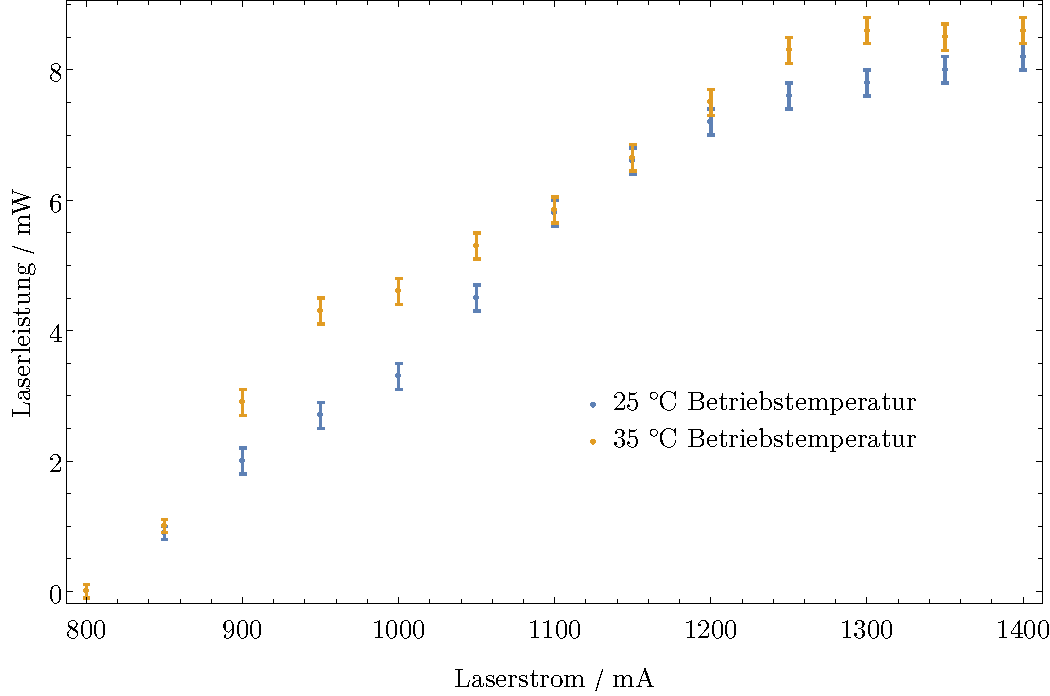
\includegraphics[width=\textwidth]{PI_gelb.pdf}
  \caption{PI-Kennlinie des gelben Lasers bei 25\grad und 35\grad
  Betriebstemperatur.}
  \label{img:PI_gelb}
\end{center}
\end{figure}



\subsubsection{Selektion über doppelbrechenden Kristall}


\paragraph{Aufbau und Durchführung}
blabla

\paragraph{Auswertung}
blabla

\begin{figure}[H]
\begin{center}
  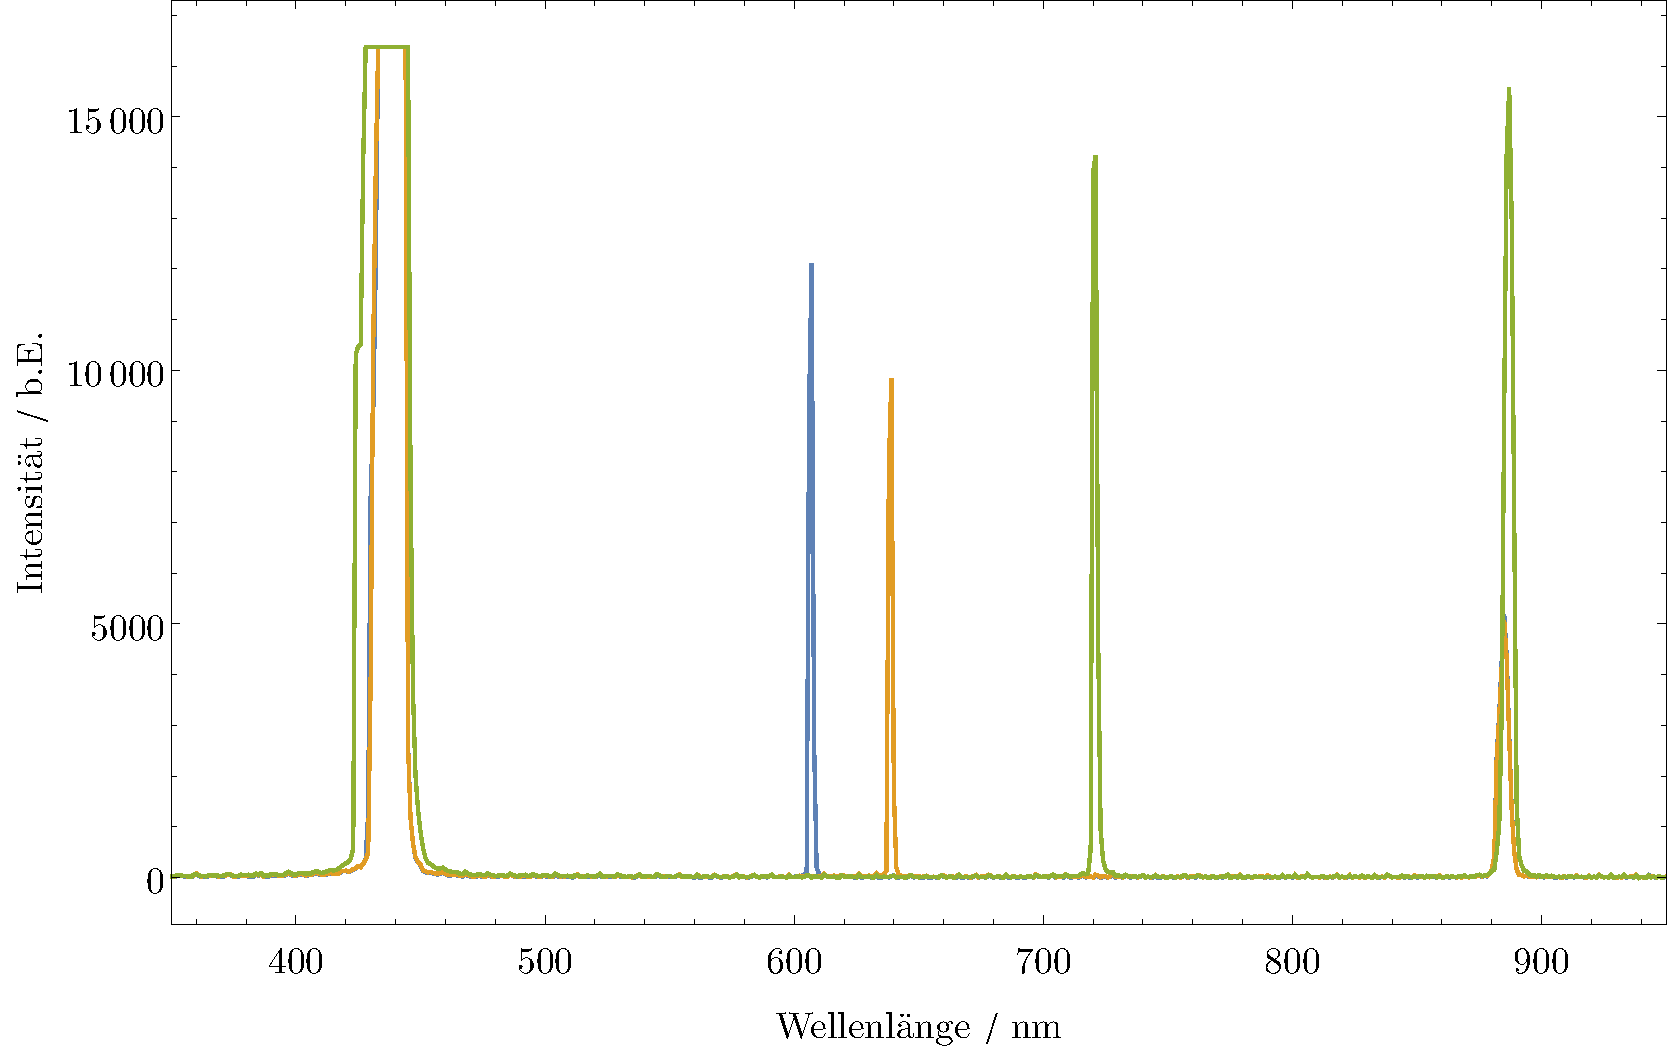
\includegraphics[width=\textwidth]{BifrSpekt.pdf}
  \caption{Spektren des Lasers für drei unterschiedliche Winkel des doppelbrechenden Kristalls.}
  \label{img:BifrSpekt}
\end{center}
\end{figure}

\subsubsection{Selektion mit Littrow-Prisma}

\paragraph{Aufbau und Durchführung}
blabla


\paragraph{Auswertung}

%an ab 0°
%max: 20°, dann stärker und schwächer
%aus ab 80°
%an bei 180°
%max: 200° wird stärker und schwächer bis 260°, hört auf, fängt an bei 0°

%dunkelrote linie
%an ab 270° bis 0°
%max: 315°
%an ab 80° bis 170°
%max bei 110°

\begin{figure}[H]
\begin{center}
  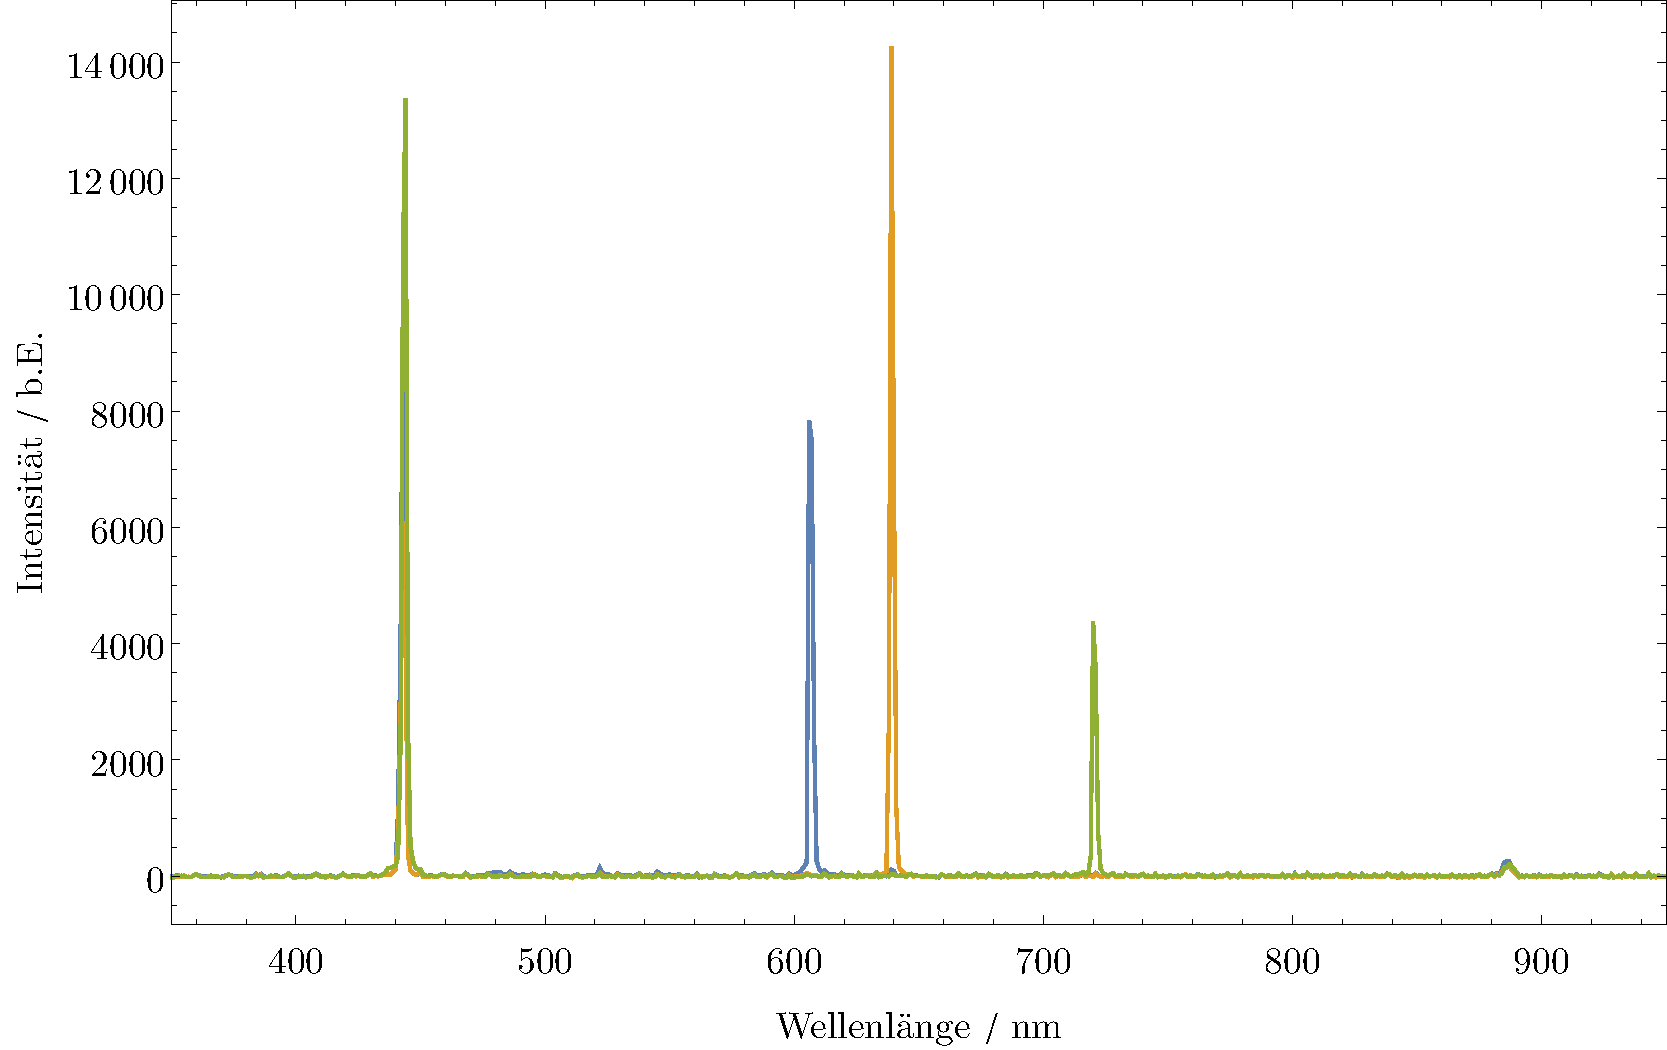
\includegraphics[width=\textwidth]{LittrSpekt.pdf}
  \caption{Spektren des Lasers für drei unterschiedliche Einstellungen des Littrow-Prismas.}
  \label{img:LittrSpekt}
\end{center}
\end{figure}

\section{Zusammenfassung und Diskussion}

\subsection{Charakterisierung des Pumplasers}

Bei der Charakterisierung des Pumplasers wurde eine Erhöhung der Laserschwelle von
$124.7\pm1.0$\,mA bei 25\grad Betriebstemperatur auf $133.0\pm1.0$\,mA bei 35\grad festgestellt.
Die Effizienz nimmt von $1.730\pm0.005$\,mW\,/\,mA auf $1.699\pm0.005$\,mW\,/\,mA ab.
Diese Messwerte entsprechen unseren Erwartungen.

Die Chiquadrat/DoF-Werte der beiden Fits liegen bei 1.6 und 0.7.
Die Abweichung vom Wert 1 kommt vermutlich daher,
dass die Fehler auf die einzelnen Messwerte aus der beobachteten Schwankung der Anzeige des
Leistungsmesskopfes abgeschätzt wurden und diese Abschätzung sehr ungenau war.
Eine genauere Analyse der Messungenauigkeit des Leistungsmesskopfes hätte hier durchgeführt werden
können, war aber für das Versuchsziel nicht relevant.
Der Fit der Kennlinie im Bereich zwischen 150\,mA und 700\,mA mit einer linearen Funktion erscheint
durch die Chiquadrat/DoF-Werte also gerechtfertigt.

Eine interessante Beobachtung ist das Überkreuzen der beiden Kennlinien bei 900\,mA;
über diesem Wert hat der Laser bei 35\grad eine höhere Leistung als bei 25\grad.

\subsection{Charakterisierung des Pr:YLF-Kristalls}

\subsubsection{Absorptionsspektrum}

Die Zuordnung einiger Linien des Absorptionsspektrums ist mit Hilfe von spektroskopischen Daten
(Tab.~\ref{tab:AbsSpecTh}) möglich.
Die Linien 2-6 können so fünf Übergängen aus dem Grundzustand zugeordnet werden
(Tab.~\ref{tab:AbsSpecVgl}).
Die systematische Abweichung der Wellenlängen um ca. 10\,nm könnte dadurch verursacht werden,
dass das Praseodym nicht in Reinform, sondern in den Pr:YLF-Kristall eingebettet vorliegt.

Die erste Absorptionsspitze bei 402\,nm lässt sich keinem Übergang von Praseodym zuordnen.
Die Form der Spitze (asymmetrisch, langsamer Abfall am rechten Rand) deutet darauf hin,
dass es sich hier um ein Artefakt handelt und nicht um eine Linie.

Die Linien 7-9 können ebenfalls nicht Praseodym zugeordnet werden.
Es könnte sich hier um Absorptionen von Li$^+$ oder F$^-$ handeln.


\begin{table}[htb]
\caption{Übergänge aus dem Grundzustand $^3$H$_4$ in angeregte Zustände von Pr$^{3+}$
\cite{NIST_ASD}.}
\begin{center}
\begin{tabular}{|c|c|c|}
\hline
Zielniveau & Wellenzahl / cm$^{-1}$ & Wellenlänge / nm \\ \hline
$^3$H$_5$ & 2152.09 & 4646.65 \\ \hline
$^3$H$_6$ & 4389.09 & 2278.38 \\ \hline
$^3$F$_2$ & 4996.61 & 2001.36 \\ \hline
$^3$F$_3$ & 6415.24 & 1558.79 \\ \hline
$^3$F$_4$ & 6854.75 & 1458.84 \\ \hline
$^1$G$_4$ & 9921.24 & 1007.94 \\ \hline
$^1$D$_2$ & 17334.4 & 576.888 \\ \hline
$^3$P$_0$ & 21389.8 & 467.512 \\ \hline
$^3$P$_1$ & 22007.5 & 454.391 \\ \hline
$^3$P$_2$ & 23160.6 & 431.768 \\ \hline
$^1$I$_6$ & 22211.5 & 450.216 \\ \hline
\end{tabular}
\end{center}
\label{tab:AbsSpecTh}
\end{table}

\begin{table}[htb]
\caption{Zuweisung der gemessenen Absorptionslinien zu Übergängen in angeregte Zustände
von~Pr$^{3+}$.}
\begin{center}
\begin{tabular}{|c|c|c|}
\hline
  & gem. Wellenlänge / nm & th. Wellenlänge / nm \\ \hline
1 & 402 & Artefakt \\ \hline
2 & 442 & 432 ($^3$P$_2$) \\ \hline
3 & 459 & 450 ($^1$I$_6$) \\ \hline
4 & 467 & 454 ($^3$P$_1$) \\ \hline
5 & 479 & 468 ($^3$P$_0$) \\ \hline
6 & 585 & 577 ($^1$D$_2$) \\ \hline
7 & 595 &  \\ \hline
8 & 886 &  \\ \hline
9 & 935 &  \\ \hline
\end{tabular}
\end{center}
\label{tab:AbsSpecVgl}
\end{table}

\FloatBarrier

\subsubsection{Emissionsspektrum}

\begin{table}[htb]
\caption{Zuweisungen der Linien des gemessenen Emissionsspektrums zu den Übergängen von~Pr$^{3+}$.}
\begin{center}
\begin{tabular}{|c|c|c|}
\hline
  & gem. Wellenlänge / nm & th. Wellenlänge / nm \cite{Versuchsanleitung} \\ \hline
1 & 442 & Pumplaserlicht \\ \hline
2 & 480 & 480 ($^3$P$_0$ $\rightarrow$ $^3$H$_4$) \\ \hline
3 & 522 & 523 ($^3$P$_1$ $\rightarrow$ $^3$H$_5$) \\ \hline
4 & 546 &  \\ \hline
5 & 587 &  \\ \hline
6 & 604 & 607 ($^3$P$_0$ $\rightarrow$ $^3$H$_6$) \\ \hline
7 & 639 & 640 ($^3$P$_0$ $\rightarrow$ $^3$F$_2$) \\ \hline
8 & 670 &  \\ \hline
9 & 697 & 689? ($^3$P$_0$ $\rightarrow$ $^3$F$_3$) \\ \hline
10 & 720 & 721 ($^3$P$_0$ $\rightarrow$ $^3$F$_4$) \\ \hline
11 & 962 &  \\ \hline
12 & 1047 &  \\ \hline
\end{tabular}
\end{center}
\label{tab:EmSpecVgl}
\end{table}

In Tab.~\ref{tab:EmSpecVgl} werden einige Linien des Emissionsspektrums mit Übergängen von Pr$^{3+}$
identifiziert.
Das Emissionsspektrum ist deutlich komplexer als das Absorptionsspektrum,
da der angeregte Zustand $^3$P$_2$ über viele verschiedene Niveaus in den Grundzustand übergehen
kann.
Einige Linien werden daher nicht zugeordnet.
Bei der ersten Linie handelt es sich entweder um gestreutes Licht des Pumplasers oder um den
direkten Übergang aus dem angeregten Zustand in den Grundzustand.

Die Übereinstimmung unserer Messdaten mit den Literaturwerten ist gut,
nur bei der 9. Linie besteht eine größere Abweichung (8\,nm).



\subsubsection{Messung der Lebensdauer des angeregten Zustands}

Diskussion chiquadrat von Lebensdauermessung, Vergleich von Lebensdauer mit Literaturwert

höhere Absorption durch Verstimmung des Pumplasers mit Temperatur und Strom?

\subsubsection{Messung der absorbierten Leistung}

\subsection{Charakterisierung des Lasers auf der roten Linie}
Hohe Chiquadrate erklären. Instabiler Betrieb, Modensprünge..?


\subsection{Wellenlängenselektion}




\newpage
\bibliographystyle{plain}
\bibliography{refs}

\newpage
\appendix

\section{Appendix}

\subsection{Verbesserungsvorschläge}

Änderungen Skript:

Laser leich kollimieren in Power meter

Seite 2: YLF: Yttrium-Lithium-Fluorid-Kristall

Abb.~8: Transmissions- und Absorptionsspektrum vertauscht

Abb.~3: $^3$P$_0 \rightarrow\,^3$F$_3$ ist hier mit 689\,nm angegeben, in Abb.~5 mit 698\,nm.

Abb.~5: $^3$P$_0 \rightarrow\,^3$F$_2$ ist zweimal vorhanden



%\clearpage
%\includepdf[pages={-}, pagecommand=\subsection{Lab log}]{../img/LabLog.pdf}

\end{document}
